\section{Proof of semantic preservation}
\label{sec:proof}

The semantic preservation property of the HM2T is expressed by a
\textit{forward simulation} theorem, which general form is as follows
(according to \cite{Leroy2009}):
\begin{equation*}
  \forall{}S,C,B,\mathtt{transf}(S)=C\land{}S\Downarrow{}B\Rightarrow{}\exists{}B'~s.t.~C\Downarrow{}B'\land{}B\sim{}B'.
\end{equation*}

Considering the above theorem in a more general framework than the one
of compilers from programming languages (which is the framework of
\cite{Leroy2009}), $S$ corresponds to an instance of a source
formalism, and $C$ is the result of the transformation of $S$ by the
transformation function $\mathtt{transf}$; $C$ is an instance of a
target formalism. $B$ and $B'$ are behaviors, and the binary relation
$\Downarrow$ states that a given instance of a formalism has a given
behavior. $B\sim{}B'$ states that the behavior $B$ is similar to the
behavior $B'$ considering a contextual definition of the similarity
relation. The forward simulation theorem must be read as follows: for
all instance $S$ of a source formalism transformed into $C$ by
function $\mathtt{transf}$, if $S$ has a behavior $B$, then $C$ has a
behavior $B'$ that is similar to $B$. In our case, we have proved a
slightly different theorem, which has the following form:
\begin{equation*}
  \forall{}S,C,B,B',~\mathtt{transf}(S)=C\land{}S\Downarrow{}B\land{}C\Downarrow{}B'\Rightarrow{}B\sim{}B'.
\end{equation*}
In the above form, we consider that the target $C$ has the behavior
$B'$, and we no more have to prove the existence of such a behavior.
This version of the theorem focuses on the behavior similarity. Thus,
we refer to it has a behavior (or trace) similarity theorem. In our
work perspectives, we contrive to prove the first form of the theorem,
but in this article we will present the proof of the second form.

In our specific transformation case, $S$ is a SITPN model and $C$ is a
\hvhdl{} design. The behavior of a SITPN model and a \hvhdl{} design
corresponds to the execution trace computed through a certain number
of clock cycles w.r.t. semantics rules that have been presented in
Sections~\ref{subsec:hpn-particularities} and
\ref{subsec:sim-semantics}. Thus, the property of semantic
preservation for the HM2T is about comparing the execution traces of
the input SITPN model and the output \hvhdl{} design. Specifically, we
want to show that, no matter how much clock cycles are performed, the
execution traces are always
\textit{similar}. Figure~\ref{fig:trace-comparison} illustrates the
comparison of the execution traces of a SITPN model input of the HM2T
and its corresponding output design.
\begin{figure}[!ht]
  \centering
  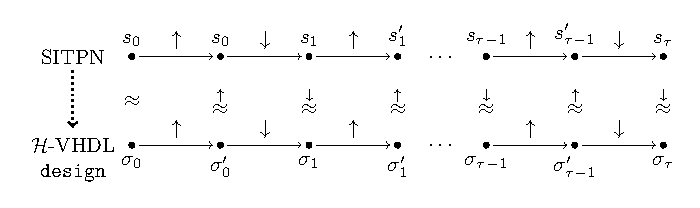
\includegraphics[keepaspectratio,width=\textwidth]{trace-comparison-full.eps}
  \caption{Comparison between the execution trace of a SITPN model (on
    the upper part) and the execution trace of the \hvhdl{} design
    resulting from the HM2T (on the lower part). The $\uparrow$
    (resp. $\downarrow$) symbol represents a rising (resp. falling)
    edge step happening in the course of a clock cycle. The $\approx$
    symbol represents the similarity relation between the upper SITPN
    state and the lower \hvhdl{} design state.}
  \label{fig:trace-comparison}
\end{figure}

In Figure~\ref{fig:trace-comparison}, $\tau$ indicates an arbitrary
number of clock cycles. To perform the proof of semantic preservation,
we must prove that every pair of states considered at the same time
point are similar w.r.t. to our own similarity relation.  Let us
introduce our general similarity criterions between a SITPN state and
a \hvhdl{} state through the relation presented in
Definition~\ref{def:state-sim}.

\begin{definition}[State similarity relation]
  \label{def:state-sim}
  For a given $sitpn\in{}SITPN$, a \hvhdl{} design $d\in{}design$, and
  a binder $\gamma\in{}WM(sitpn,d)$, an SITPN state $s\in{}S(sitpn)$
  and a design state $\sigma\in\Sigma$ are similar, written
  $\gamma\vdash{}s\approx\sigma$ if
  \begin{enumerate}
  \item\label{item:sim-mark} $\forall{}p\in{}P,$
    $~s.M(p)=\sigma(\gamma(p))($\texttt{s\_marking}$)$.
  \item\label{item:sim-tc}
    $\forall{}t\in{}T_i,$\\
    $\big(u(I_s(t))=\infty\land{}s.I(t)\le{}l(I_s(t))\Rightarrow{}s.I(t)=\sigma(\gamma(t))($\texttt{s\_time\_counter}$)\big)$\\
    $\land\big(u(I_s(t))=\infty\land{}s.I(t)>{}l(I_s(t))\Rightarrow{}\sigma(\gamma(t))($\texttt{s\_time\_counter}$)=l(I_s(t))\big)$\\
    $\land\big(u(I_s(t))\neq\infty\land{}s.I(t)>{}u(I_s(t))\Rightarrow{}\sigma(\gamma(t))($\texttt{s\_time\_counter}$)=u(I_s(t))\big)$\\
    $\land\big(u(I_s(t))\neq\infty\land{}s.I(t)\le{}u(I_s(t))\Rightarrow{}s.I(t)=\sigma(\gamma(t))($\texttt{s\_time\_counter}$)\big)$.
  \item\label{item:sim-reset} $\forall{}t\in{}T_i,$
    $s.reset_t(t)=\sigma(\gamma(t))($\texttt{s\_reinit\_time\_counter}$)$.
  \item\label{item:sim-cond}
    $\forall{}c\in\mathcal{C},~s.cond(c)=\sigma(\gamma(c))$.
  \item\label{item:sim-act}
    $\forall{}a\in\mathcal{A},~s.ex(a)=\sigma(\gamma(a))$.
  \item\label{item:sim-fun}
    $\forall{}f\in\mathcal{F},~s.ex(f)=\sigma(\gamma(f))$.
  \end{enumerate}
\end{definition}

In Definition~\ref{def:state-sim}, the binder structure $\gamma$ that
is generated by the HM2T relates the elements of the SITPN model to
the elements of the \hvhdl{} design, and thus enables the comparison
between the SITPN state and the design state. In
Definition~\ref{def:state-sim}, Point~\ref{item:sim-mark} relates the
marking value of a place $p$ at state $s$ to the value of the
\texttt{s\_marking} signal, which is an internal signal of the PDI
identified by $\gamma(p)$. Here, the expression $\sigma(\gamma(p))$
returns the internal state of the PDI $\gamma(p)$ by looking up the
component store of state $\sigma$. Point~\ref{item:sim-tc} (resp.
Point~\ref{item:sim-reset} similarly relate the value of time counters
(resp. reset orders) of transitions to the value of the
$\texttt{s\_time\_counter}$ signal
(resp. $\texttt{s\_reinit\_time\_counter}$) in the internal state of
the corresponding TDIs. In Point~\ref{item:sim-cond}
(resp. \ref{item:sim-act} and \ref{item:sim-fun}), the Boolean value
of conditions (resp. actions and functions) are compared to the value
of the input (resp. output) ports of the output design, also based on
the $\gamma$ binder.  As one can observe in Point~\ref{item:sim-tc},
due to the specific implementation of time intervals with an infinite
upper bound in \hvhdl{}, the relation between the value of a time
counter and the value of the $\texttt{s\_time\_counter}$ signal can
not be restricted to a simple equality.

As shown in Figure~\ref{fig:trace-comparison}, we make a distinction
between the state similarity after a rising edge phase and after a
falling edge phase. The definitions of the post rising edge similarity
relation, written $\stackrel{\uparrow}{\approx}$, and the post falling
edge similarity relation, written $\stackrel{\uparrow}{\approx}$, are
restrictions of the general definition. After a rising edge phase, the
equality between the value of conditions and the value of condition
ports (i.e. Point~\ref{item:sim-cond} of
Definition~\ref{def:state-sim}) does not hold, and after a falling
edge phase, the equality between the value of time counter reset
orders and the value of the \texttt{s\_reinit\_time\_counter} signals
(i.e. Point~\ref{item:sim-reset} of Definition~\ref{def:state-sim})
does not hold. However, these divergences do not impact the
computation logic of the overall so that to create further behavioral
divergences between the input SITPN model and the output \hvhdl{}
design.

Definition~\ref{def:exec-trace-sim} introduces the relation that
states that a SITPN model's execution trace is similar to a \hvhdl{}
design's execution trace.

\begin{definition}[Execution trace similarity]
  \label{def:exec-trace-sim}
  For a given $sitpn\in{}SITPN$, a \hvhdl{} design $d\in{}design$, and
  a binder $\gamma\in{}WM(sitpn,d)$, the execution trace
  $\theta_s\in{}\mathtt{list}(S(sitpn))$ and the simulation trace
  $\theta_\sigma\in\mathtt{list}(\Sigma)$ are similar, written
  $\gamma\vdash{}\theta_s\stackrel{clk}{\sim}\theta_\sigma$ where
  $clk\in\{\uparrow,\downarrow\}$, according to the following rules:\\

  \begin{tabular}{@{}l}
    {\begin{prooftree}[template={\inserttext}]        
        \infer0[$clk\in{}\{\uparrow,\downarrow\}$]{$\gamma\vdash{}[~]\stackrel{clk}{\sim}{}[~]$}
      \end{prooftree}} 
  \end{tabular}
  \begin{tabular}{@{}l}
    {\begin{prooftree}[template={\inserttext}]

        \hypo{$\gamma\vdash{}s\stackrel{\uparrow}{\sim}\sigma$}
        \hypo{$\gamma\vdash{}\theta_s\stackrel{\downarrow}{\sim}{}\theta_\sigma$}
        \infer2{$\gamma\vdash{}(s :: \theta_s)\stackrel{\uparrow}{\sim}{}(\sigma :: \theta_\sigma)$}
      \end{prooftree}} 
  \end{tabular}
  \begin{tabular}{@{}l}
    {\begin{prooftree}[template={\inserttext}]

        \hypo{$\gamma\vdash{}s\stackrel{\downarrow}{\sim}\sigma$}
        \hypo{$\gamma\vdash{}\theta_s\stackrel{\uparrow}{\sim}{}\theta_\sigma$}
        \infer2{$\gamma\vdash{}(s :: \theta_s)\stackrel{\downarrow}{\sim}{}(\sigma :: \theta_\sigma)$}
      \end{prooftree}} 
  \end{tabular}
\end{definition}

In Definition~\ref{def:exec-trace-sim}, the clock event symbol on top
of the $\sim$ sign indicates the kind of clock event that led to the
production of the states at the head of the traces. The execution
trace similarity relation expects that the states composing the traces
have been alternatively produced by a rising edge step followed by a
falling edge step. By construction, the traces must have the same
length to respect the execution trace similarity relation.

To handle the case of an execution/simulation trace beginning by an
initial state, that is, a state neither reached after a rising nor
after a falling edge, we give a slightly different definition of the
execution trace similarity relation in
Definition~\ref{def:full-exec-trace-sim}.

\begin{definition}[Full execution trace similarity]
  \label{def:full-exec-trace-sim} For a given $sitpn\in{}SITPN$, a
  \hvhdl{} design $d\in{}design$, and a binder
  $\gamma\in{}WM(sitpn,d)$, the execution trace
  $\theta_s\in{}\mathtt{list}(S(sitpn))$ and the simulation trace
  $\theta_\sigma\in\mathtt{list}(\Sigma)$ are fully similar, written
  $\gamma\vdash{}\theta_s\sim\theta_\sigma$, according to the
  following rules:\\

  \begin{tabular}{l}
    {\begin{prooftree}[template={\inserttext}]
        \infer0{$\gamma\vdash{}[~]\sim{}[~]$}
      \end{prooftree}}
  \end{tabular}
  \begin{tabular}{l}
    {\begin{prooftree}[template={\inserttext}]

        \hypo{$\gamma\vdash{}s\sim\sigma$}
        \hypo{$\gamma\vdash{}\theta_s\stackrel{\uparrow}{\sim}{}\theta_\sigma$}
        \infer2{$\gamma\vdash{}(s :: \theta_s)\sim{}(\sigma ::
          \theta_\sigma)$}
      \end{prooftree}}
  \end{tabular}
\end{definition}

The full execution trace similarity relation indicates that the head
states of traces must verify the general state similarity relation
(cf. Figure~\ref{fig:trace-comparison}), and that the tail of the
traces must respect the execution state similarity relation starting
with a rising edge step.

Now, let us introduce the necessary lemmas to prove the semantic
preservation theorem. In Definition~\ref{def:hm2t-hyps}, we present
the hypotheses expressing the fact that we are proving the semantic
preservation property for the HM2T. These hypotheses will always
appear in the lemmas and theorems presented afterwards.

\begin{definition}[HM2T hypotheses]
  \label{def:hm2t-hyps}
  For all well-defined $sitpn\in{}SITPN$, bounding function
  $b\in{}P\rightarrow\mathbb{N}$, \hvhdl{} design $d\in{}design$,
  binder $\gamma\in{}WM(sitpn,d)$, elaborated design
  $\Delta\in{}ElDesign$, default state $\sigma_e\in\Sigma$, simulation
  environment $E_p\in\mathbb{N}\rightarrow{}(id\nrightarrow{}v)$, and
  execution environment
  $E_c\in\mathbb{N}\rightarrow(\mathcal{C}\rightarrow\mathbb{B})$,
  assume that:
  \begin{enumerate}
  \item\label{it:HM2T-some} Taking the SITPN model $sitpn$ and the
    bounding function $b$ as inputs, the HM2T returns an output design
    $d$ and a binder $\gamma$, written
    $\mathtt{sitpn2hvhdl}(sitpn, b)=\lfloor(d,\gamma)\rfloor$ where
    $\mathtt{sitpn2hvhdl}\in{}SITPN\rightarrow(P\rightarrow\mathbb{N})\nrightarrow(design\times{}WM(sitpn,d))$.
  \item\label{it:sitpn-is-bounded} $sitpn$ is bounded through $b$,
    written $\lceil{}sitpn\rceil^b$.
  \item In the context of the \hilecop{} design store
    $\mathcal{D}_\mathcal{H}$ and with an empty generic constant
    dimensioning function ($\emptyset$), $d$ is elaborated into
    $\Delta$ with a default state $\sigma_e$, written
    $\mathcal{D}_\mathcal{H},\emptyset\vdash{}d\xrightarrow{elab}\Delta,\sigma_e$.
  \item\label{it:env-are-sim} Simulation and execution environments
    are similar, written $\gamma\vdash{}E_p\stackrel{env}{=}E_c$.
  \end{enumerate}
  
\end{definition}

In Point~\ref{it:HM2T-some} of Definition~\ref{def:hm2t-hyps}, the
$\mathtt{sitpn2hvhdl}$ function implements the HM2T, that is a
function proved sound and complete w.r.t. to the specification
presented in Section~\ref{sec:m2t}. Point~\ref{it:sitpn-is-bounded}
expresses the boundedness property of the input SITPN
model. Point~\ref{it:env-are-sim} states that, at each time point, the
execution and simulation environments yield the same Boolean value for
all couple condition-condition port linked through $\gamma$.

\def\hm2thyps{well-defined $sitpn\in{}SITPN$,
  $b\in{}P\rightarrow\mathbb{N}$, $d\in{}design$,
  $\gamma\in{}WM(sitpn,d)$, $\Delta\in{}ElDesign,\sigma_{e}\in\Sigma$,
  $E_p\in\mathbb{N}\rightarrow{}(id\nrightarrow{}v)$, and
  $E_c\in\mathbb{N}\rightarrow(\mathcal{C}\rightarrow\mathbb{B})$ that
  verify the hypotheses of Definition~\ref{def:hm2t-hyps}}

As illustrated in Figure~\ref{fig:trace-comparison}, to prove that the
execution traces are similar, we must first prove that the two initial
states are similar. This is expressed by
Lemma~\ref{lem:sim-init-states}.
\begin{lemma}[Similar initial states]
  \label{lem:sim-init-states}
  For all \hm2thyps{}, and for all $\sigma_0,\sigma_i\in{}\Sigma$ such that:
  \begin{itemize}
  \item $\sigma_0$ is the initial state of design $d$:\\
    $\mathcal{D},\Delta,\sigma_e\vdash{}d.beh\xrightarrow{cs_i}{}\sigma_i$ and
    $\mathcal{D},\Delta,\sigma_i\vdash{}d.beh\xrightarrow{\rightsquigarrow}{}\sigma_0$
  \end{itemize}
  then $\gamma\vdash{}s_0\approx\sigma_0$.
\end{lemma}

Starting from two similar initial states, then we must prove that each
phase, or step, of a clock cycle produces still similar states.  This
is expressed by \textit{lock-step simulation} lemmas \cite{Leroy2009},
which are of the following form in their \textit{non-existantial}
version:
\begin{equation*}
  \forall{}S_1,S'_1,S_2,S'_2,~S1\rightarrow{}S'_1\land{}S_2\rightarrow{}S'_2\land{}S_1\approx{}S_2\Rightarrow{}S'_1\approx{}S'_2.
\end{equation*}
Here, $S_1$ and $S'_1$ are two states of the source formalism, $S_2$
and $S'_2$ are two states of the target formalism.
$S_1\rightarrow{}S'_1$ (resp. $S_2\rightarrow{}S'_2$) states that an
execution step leads from $S_1$ to $S'_1$ (resp. from $S_2$ to $S'_2$)
w.r.t. a contextual definition of the execution
step. $S_1\approx{}S_2$ indicates that $S_1$ and $S_2$ are similar,
also w.r.t. a contextual definition of state similarity. The above
theorem must be read as follows: given two similar states $S_1$ and
$S_2$, if one execution step leads from $S_1$ to $S'_1$ and from $S_2$
to $S'_2$, then $S'_1$ and $S'_2$ are similar. \\

To establish the semantic preservation property, the first lock-step
simulation lemma that we had to prove pertains to the first rising
edge step. As defined in the SITPN semantics, the first rising edge
step is idle, i.e. a SITPN model is still in its initial state after
this step. Thus, we must prove that the state of the output design
reached after the first rising edge is similar to the SITPN model's
initial state. This is expressed by Lemma~\ref{lem:fst-re-lock-step}.

\begin{lemma}[First rising edge lock-step simulation]
  \label{lem:fst-re-lock-step}
  For all \hm2thyps{}, and for all clock count $\tau\in\mathbb{N}$,
  $\sigma_0,\sigma_i,\sigma_{\uparrow},\sigma'_0\in{}\Sigma$ such that:
  \begin{itemize}
  \item $\sigma_0$ is the initial state of design $d$:\\
    $\mathcal{D},\Delta,\sigma_e\vdash{}d.beh\xrightarrow{cs_i}{}\sigma_i$ and
    $\mathcal{D},\Delta,\sigma_i\vdash{}d.beh\xrightarrow{\rightsquigarrow}{}\sigma_0$
    
  \item a rising edge step leads from $\sigma_0$ to $\sigma'_0$:\\
    $\mathcal{D}_\mathcal{H},\Delta,\mathtt{inj}(\sigma_0,E_p,\tau)\vdash{}d.beh\xrightarrow{cs_{\uparrow}}\sigma_{\uparrow}$
    and
    $\mathcal{D}_\mathcal{H},\Delta,\sigma_{\uparrow}\vdash{}d.beh\xrightarrow{\rightsquigarrow}\sigma'_0$
  \end{itemize}
  then $\gamma\vdash{}s_0\stackrel{\uparrow}{\approx}\sigma'_0$.
\end{lemma}
In Lemma~\ref{lem:fst-re-lock-step}, $s_0$ is the initial state of the
SITPN model as introduced in
Definition~\ref{def:sitpn-init-state}.  Note that a rising edge step on the \hvhdl{} side refers to the conjunction of the three following phases: the injection of fresh values in primary input ports (through the use of the \texttt{inj} function), the execution of rising blocks, and the stabilization of combinational parts. \\

Then, we must prove that any rising edge or falling edge step verifies
the lock-step simulation property. This is expressed by
Lemmas~\ref{lem:re-lock-step} and \ref{lem:fe-lock-step}. 

\begin{lemma}[Rising edge lock-step simulation]
  \label{lem:re-lock-step}
  For all \hm2thyps{}, and for all $\tau\in\mathbb{N}$,
  $s,s'\in{}S(sitpn)$, $\sigma,\sigma_\uparrow,\sigma'\in\Sigma$, such
  that
  \begin{itemize}
  \item $s$ and $\sigma$ are similar states as intended after a
    falling edge step:
    $\gamma\vdash{}s\stackrel{\downarrow}{\approx}\sigma$
  \item a rising edge step leads from $s$ to $s'$:
    $E_c,\tau\vdash{}s\xrightarrow{\uparrow}s'$
  \item a rising edge step leads from $\sigma$ to $\sigma'$:\\
    $\mathcal{D}_\mathcal{H},\Delta,\mathtt{inj}(\sigma,E_p,\tau)\vdash{}d.beh\xrightarrow{cs_{\uparrow}}\sigma_{\uparrow}$
    and
    $\mathcal{D}_\mathcal{H},\Delta,\sigma_{\uparrow}\vdash{}d.beh\xrightarrow{\rightsquigarrow}\sigma'$
  \end{itemize}
  then $\gamma\vdash{}s'\stackrel{\uparrow}{\approx}{}\sigma'$.
  
\end{lemma}

\begin{lemma}[Falling edge lock-step simulation]
  \label{lem:fe-lock-step}
  For all \hm2thyps{}, and for all $\tau\in\mathbb{N}$,
  $s,s'\in{}S(sitpn)$, $\sigma,\sigma_\downarrow,\sigma'\in\Sigma$,
  such that
  \begin{itemize}
  \item $s$ and $\sigma$ are similar states as intended after a rising
    edge step: $\gamma\vdash{}s\stackrel{\downarrow}{\approx}\sigma$
  \item a falling edge step leads from $s$ to $s'$:
    $E_c,\tau\vdash{}s\xrightarrow{\downarrow}s'$
  \item a falling edge step leads from $\sigma$ to $\sigma'$:\\
    $\mathcal{D}_\mathcal{H},\Delta,\sigma\vdash{}d.beh\xrightarrow{cs_{\downarrow}}\sigma_{\downarrow}$
    and
    $\mathcal{D}_\mathcal{H},\Delta,\sigma_{\downarrow}\vdash{}d.beh\xrightarrow{\rightsquigarrow}\sigma'$
  \end{itemize}
  then $\gamma\vdash{}s'\stackrel{\downarrow}{\approx}{}\sigma'$.
\end{lemma}

As expressed in Lemma~\ref{lem:fe-lock-step}, a falling edge step on
the \hvhdl{} side refers to the execution of falling blocks followed
by the stabilization of combinational parts.\\

Under the assumptions of Lemma~\ref{lem:sim-init-states},
\ref{lem:fst-re-lock-step}, \ref{lem:re-lock-step} and
\ref{lem:fe-lock-step}, we can now prove the following trace
similarity theorem expressing that the HM2T is semantic preserving.

\begin{theorem}[Full trace similarity]
  \label{thm:full-trace-sim}
  For all well-defined $sitpn\in{}SITPN$, bounding function
  $b\in{}P\rightarrow\mathbb{N}$, \hvhdl{} design $d\in{}design$,
  binder $\gamma\in{}WM(sitpn,d)$, default state $\sigma_e\in\Sigma$,
  simulation environment
  $E_p\in\mathbb{N}\rightarrow{}(id\nrightarrow{}v)$, execution
  environment
  $E_c\in\mathbb{N}\rightarrow(\mathcal{C}\rightarrow\mathbb{B})$,
  $\tau\in\mathbb{N}$, SITPN model trace
  $\theta_s\in\mathtt{list}(S(sitpn))$, and \hvhdl{} design trace
  $\theta_\sigma\in\mathtt{list}(\Sigma)$ such that:
  \begin{enumerate}
  \item $\mathtt{sitpn2hvhdl}(sitpn, b)=\lfloor(d,\gamma)\rfloor$
  \item $\lceil{}sitpn\rceil^b$
  \item $\gamma\vdash{}E_p\stackrel{env}{=}E_c$
  \item $E_c,\tau\vdash{}sitpn\xrightarrow{full}\theta_s$
  \item
    $\mathcal{D}_\mathcal{H},\emptyset,E_p,\tau\vdash{}d\xrightarrow{full}\theta_\sigma$
  \end{enumerate}
  then $\gamma\vdash\theta_s\sim\theta_\sigma$.
\end{theorem}

\begin{pf}[Proof of Theorem~\ref{thm:full-trace-sim}.]
  
  Proceeding by case analysis on the number of clock cycles $\tau$,
  there are two cases. First $\tau=0$, and then we must prove that the
  initial states are similar, which is true appealing to
  Lemma~\ref{lem:sim-init-states}. Otherwise, $\tau>0$ and then at
  least the first clock cycle is executed. Thanks to
  Lemmas~\ref{lem:fst-re-lock-step} and \ref{lem:fe-lock-step}, we can
  show that the states are similar during the first clock cycle. Then,
  we can reason by induction over $\tau$ to prove that the remnant of
  the execution traces are similar. We can appeal to
  Lemmas~\ref{lem:re-lock-step} and \ref{lem:fe-lock-step} to prove
  that states are similar during the induction step (corresponding to
  an arbitrary clock cycle step), and then use the induction
  hypothesis to complete the proof.

\end{pf}

\subsection{A mechanization-ready proof}
\label{sec:mecha-ready-pf}

As presented above, proving Theorem~\ref{thm:full-trace-sim} amounts
to proving Lemma~\ref{lem:sim-init-states}, which is about the
similarity of the initial states, and the different lock-step
simulation lemmas (i.e. Lemmas~\ref{lem:fst-re-lock-step},
\ref{lem:re-lock-step} and \ref{lem:fe-lock-step}). Preparing for the
mechanization of the proof of Theorem~\ref{thm:full-trace-sim} with
the \coq{} proof assistant, we have written very detailed proof (a
hundred-page long) for Lemmas~\ref{lem:sim-init-states},
\ref{lem:fst-re-lock-step}, \ref{lem:re-lock-step} and
\ref{lem:fe-lock-step}. The full proof is available in
\cite{Iampietro2021}. Even though obviously a tedious task, writing
the fully detailed proof before the mechanization has been a
successful process. It has revealed a bug in the \vhdl{} code defining
the behavior of the place design, which has been corrected in the
version given in Appendix~\ref{app:place-design}.  Due to the
important amount of work demanded by the mechanization task, if we had
tackled down the mechanization of the proof without a previously
detailed proof plan, this bug would not have yet been detected. \\

To illustrate the level of details reached in our proof, let us
present an extract of the proof of
Lemma~\ref{lem:re-lock-step}. Lemma~\ref{lem:re-lock-step} states that
the rising edge step verifies the lock-step simulation property. To
prove that the states of the input SITPN model and the output design
are similar after a rising edge step, we must prove, among other
points, that the marking of each place is equal to the value the
\texttt{s\_marking} internal signal in its corresponding PDI. This is
expressed by Lemma~\ref{lem:re-eq-marking}.

\begin{lemma}[Rising edge equal marking]
  \label{lem:re-eq-marking}
  For all \hm2thyps{}, and for all $\tau\in\mathbb{N}$,
  $s,s'\in{}S(sitpn)$, $\sigma,\sigma_\uparrow,\sigma'\in\Sigma$, such
  that
  \begin{itemize}
  \item $s$ and $\sigma$ are similar states as intended after a
    falling edge step:
    $\gamma\vdash{}s\stackrel{\downarrow}{\approx}\sigma$
  \item a rising edge step leads from $s$ to $s'$:
    $E_c,\tau\vdash{}s\xrightarrow{\uparrow}s'$
  \item a rising edge step leads from $\sigma$ to $\sigma'$:\\
    $\mathcal{D}_\mathcal{H},\Delta,\mathtt{inj}(\sigma,E_p,\tau)\vdash{}d.beh\xrightarrow{cs_{\uparrow}}\sigma_{\uparrow}$
    and
    $\mathcal{D}_\mathcal{H},\Delta,\sigma_{\uparrow}\vdash{}d.beh\xrightarrow{\rightsquigarrow}\sigma'$
  \end{itemize}
  then
  $\forall{}p\in{}P,~s'.M(p)=\sigma'(\gamma(p))(\mathtt{s\_marking})$.
  
\end{lemma}

\begin{pf}[Proof of Lemma~\ref{lem:re-eq-marking}.]
  Given all the elements and assuming all the hypotheses expressed in
  Lemma~\ref{lem:re-eq-marking}, then, given a place $p\in{}P$, let us
  show that:
  \begin{equation*}
    \boxed{s'.M(p)=\sigma'(\gamma(p))(\texttt{s\_marking}).}
  \end{equation*}

  By definition of the SITPN state transition relation on rising edge
  (cf. Definition~\ref{def:semantics}, Point~\ref{it:new-marking}), we
  have:
  \begin{equation}\label{eq:re-eq-marking-eqmp}
    s'.M(p)=s.M(p)-\sum\limits_{t\in{}Fired(s)}pre(p,t)+\sum\limits_{t\in{}Fired(s)}post(t,p)
  \end{equation}

  \bigskip
  
  By definition of the HM2T (cf. Definition~\ref{def:hm2t-spec},
  Point~\ref{it:pdi-exists}), there exists $g_p,i_p,o_p$ such that
  $\mathtt{comp}(\gamma(p),\mathtt{place},g_p,i_p,o_p)\in{}d.beh$.  By
  property of the \hvhdl{} concurrent statement execution relation
  (cf. Table~\ref{tab:cs-eval}), the stabilization relation
  (cf. Table~\ref{tab:stabilization}),
  $\mathtt{comp}(\gamma(p),\mathtt{place},g_p,i_p,o_p)\in{}d.beh$, and
  through the examination of the \texttt{marking} process defined in
  the behavior of the place design (Appendix~\ref{app:place-design},
  Line~49), we can deduce that the following equation holds:
  \begin{equation}\label{eq:re-eq-marking-eqsm}
    \begin{split}
      \sigma'(\gamma(p))(\texttt{sm})=\sigma(\gamma(p))(\texttt{sm})-\sigma(\gamma(p))(\texttt{s\_output\_token\_sum})\\
      +\sigma(\gamma(p))(\texttt{s\_input\_token\_sum})
    \end{split}
  \end{equation}

  \bigskip
  
  \noindent{}Rewriting the goal with \eqref{eq:re-eq-marking-eqmp} and
  \eqref{eq:re-eq-marking-eqsm}, we must show that:
  \begin{equation*}
    \boxed{
      \begin{array}{c}
      s.M(p)-\sum\limits_{t\in{}Fired(s)}pre(p,t)+\sum\limits_{t\in{}Fired(s)}post(t,p)\\
      = \\
      \sigma(\gamma(p))(\texttt{sm})-\sigma(\gamma(p))(\texttt{sots})
      +\sigma(\gamma(p))(\texttt{sits}) \\
      \end{array}}
  \end{equation*}
  
  \bigskip
  
  By definition of the state similarity relation
  (cf. Definition~\ref{def:state-sim}, Point~\ref{item:sim-mark}), we
  can deduce that $s.M(p)=\sigma(\gamma(p))(\texttt{sm})$. Then, two
  points remain to be shown to complete the proof:
  \begin{enumerate}
  \item $\sum\limits_{t\in{}Fired(s)}pre(p,t)=\sigma(\gamma(p))(\texttt{sots})$
  \item $\sum\limits_{t\in{}Fired(s)}post(t,p)=\sigma(\gamma(p))(\texttt{sits})$
  \end{enumerate}

  \bigskip
  
  We will only detail the proof of the second point. The \texttt{sits}
  signal is an internal signal of the place design. It is a
  \textit{combinational} signal, that is, an equation relates its
  value to the value of other signals, and this equation holds at any
  moment in the execution of the design.  In the case of the
  \texttt{sits} signal, the \texttt{input\_tokens\_sum} process
  defines the related combinational equation.  Thus, by property of
  the stabilization relation (cf. Table~\ref{tab:stabilization}),
  $\mathtt{comp}(\gamma(p),\mathtt{place},g_p,i_p,o_p)\in{}d.beh$, and
  through the examination of the \texttt{input\_tokens\_sum} process
  defined in the behavior of the place design
  (Appendix~\ref{app:place-design}, Line~29), we can deduce that the
  following equation holds:
  \begin{equation}
    \label{eq:sits-at-fe}
    \sigma(\gamma(p))(\texttt{sits})=\sum\limits_{i=0}^{\Delta(\gamma(p))(\texttt{ian})-1}
    \begin{cases}
      \sigma(\gamma(p))(\texttt{iaw})[i]~\mathtt{if}~\sigma(\gamma(p))(\texttt{itf})[i]\\
      0~otherwise \\
    \end{cases}
  \end{equation}

  \noindent{}Rewriting the goal with \eqref{eq:sits-at-fe}:\\
  \begin{equation*}
    \boxed{
      \sum\limits_{t\in{}Fired(s)}post(t,p)=\sum\limits_{i=0}^{\Delta(\gamma(p))(\texttt{ian})-1}
      \begin{cases}
        \sigma(\gamma(p))(\texttt{iaw})[i]~\mathtt{if}~\sigma(\gamma(p))(\texttt{otf})[i]\\
        0~otherwise \\
      \end{cases}}
  \end{equation*}

  \bigskip
  
  \noindent{}Let us unfold the definition of the left sum term:\\
  \begin{equation*}
    \boxed{\begin{array}{c}
      \sum\limits_{t\in{}Fired(s)}
      \begin{cases}
        \omega~\mathtt{if}~post(t,p)=\lfloor\omega\rfloor \\
        0~otherwise
      \end{cases} \\
      = \\
      \sum\limits_{i=0}^{\Delta(\gamma(p))(\texttt{ian})-1}
      \begin{cases}
        \sigma(\gamma(p))(\texttt{iaw})[i]~\mathtt{if}~\sigma(\gamma(p))(\texttt{itf})[i]\\
        0~otherwise \\
      \end{cases} \\
    \end{array}}
  \end{equation*}

  \bigskip
  
  \noindent{}Let us perform case analysis on $\mathtt{input}(p)$;
  there are two cases:

  \begin{itemize}
  \item \textbf{CASE} $\mathtt{input}(p)=\emptyset$:\\
    
    By definition of the HM2T (cf. \cite{Iampietro2022hfspec} to see
    the case where $\mathtt{input}(p)=\emptyset$), we have
    $(\mathtt{ian}\Rightarrow{}1)\in{}g_p$,
    $(\mathtt{itf}(0)\Rightarrow{}\mathtt{true})\in{}i_p$, and
    $(\mathtt{iaw}(0)\Rightarrow{}0)\in{}i_p$.

    By property of the elaboration relation, and knowing that
    $\mathtt{comp}(\gamma(p),\mathtt{place},g_p,i_p,o_p)\in{}d.beh$,
    $(\mathtt{ian}\Rightarrow{}1)\in{}g_p$,
    $(\mathtt{itf}(0)\Rightarrow{}\mathtt{true})\in{}i_p$, and
    $(\mathtt{iaw}(0)\Rightarrow{}0)\in{}i_p$, we can deduce that the
    following equations hold:
    \begin{eqnarray}
      \label{eq:eq-ian-itfz-iawz-0}
      \Delta(\gamma(p))(\texttt{ian})&=&1 \\
      \label{eq:eq-ian-itfz-iawz-1}\sigma(\gamma(p))(\texttt{itf})[0]&=&\mathtt{true} \\
      \label{eq:eq-ian-itfz-iawz-2}\sigma(\gamma(p))(\texttt{iaw})[0]&=&0
    \end{eqnarray}

    By property of $\mathtt{input}(p)=\emptyset$, we can deduce:
    \begin{equation}
      \sum\limits_{t\in{}Fired(s)}
      \begin{cases}
        \omega~\mathtt{if}~post(t,p)=\lfloor\omega\rfloor \\
        0~otherwise
      \end{cases}=0.
      \label{eq:post-sum-eq-z}    
    \end{equation}

    \noindent{}Rewriting the goal with \eqref{eq:eq-ian-itfz-iawz-0},
    \eqref{eq:eq-ian-itfz-iawz-1}, \eqref{eq:eq-ian-itfz-iawz-2} and
    \eqref{eq:post-sum-eq-z}, we arrive to a tautology.\\
    
  \item \textbf{CASE} $input(p)\neq\emptyset$:\\

    By definition of the HM2T (Definition~\ref{def:hm2t-spec},
    Point~\ref{it:pdi-gmap}), we have
    $(\mathtt{ian}\Rightarrow{}\vert{}input(p)\vert)\in{}g_p$, and by
    property of the elaboration relation, we can deduce:
    \begin{equation}
      \Delta(\gamma(p))(\texttt{ian})=\vert{}input(p)\vert.\label{eq:ian-eq-input-card}
    \end{equation}

    To ease the reading, let us define functions
    $f\in{}Fired(s)\rightarrow\mathbb{N}$ and
    $g\in[0,\vert{}input(p)\vert-1]\rightarrow\mathbb{N}$ s.t. $f(t)=
    \begin{cases}
      \omega~\mathtt{if}~post(t,p)=\lfloor\omega\rfloor \\
      0~otherwise
    \end{cases}$
    and $g(i)=
    \begin{cases}
      \sigma(\gamma(p))(\texttt{iaw})[i]~\mathtt{if}~\sigma(\gamma(p))(\texttt{itf})[i]\\
      0~otherwise 
    \end{cases}$.

    \noindent{}The goal can be expressed as follows:
    \begin{equation*}
      \boxed{\sum\limits_{t\in{}Fired(s)}f(t)=\sum\limits_{i=0}^{\Delta(\gamma(p))(\texttt{ian})-1}g(i)}
    \end{equation*}
    
    \noindent{}Rewriting the goal with \eqref{eq:ian-eq-input-card}, we must show:
    \begin{equation*}
      \boxed{\sum\limits_{t\in{}Fired(s)}f(t)=\sum\limits_{i=0}^{\vert{}input(p)\vert-1}g(i)}
    \end{equation*}

    Now, we must prove the above equality between two sums. We had to
    prove a lot of such equalities during the entire proof. Thus, we
    came up with Theorem that presents a set of
    sufficient conditions to prove that two sums are equal.

    \begin{theorem}[Equality between two sums]
      \label{thm:sums-equal}
      For all sets $X,Y,A,B$ such that $A\subseteq{}X$ and
      $Y\subseteq{}X$, and for all functions
      $f\in{}A\rightarrow\mathbb{N}$, $g\in{}B\rightarrow\mathbb{N}$,
      if there exists $\beta\in{}Y\rightarrow{}B$ such that:
      \begin{itemize}
      \item $\beta$ is a bijection
      \item $\forall{}a\in{}A\cap{}Y,~f(a)=g(\beta(a))$
      \item $\forall{}a\in{}A\setminus{}Y,~f(a)=0$
      \item $\forall{}b\in{}B,\beta^{-1}(b)\notin{}A\Rightarrow{}g(b)=0$
      \end{itemize}
      then $\sum\limits_{a\in{}A}f(a)=\sum\limits_{b\in{}B}g(b)$.
    \end{theorem}
    
    By property of the HM2T, there exists a bijection
    $\beta\in\mathtt{input}(p)\rightarrow{}[0,\vert{}input(p)\vert-1]$
    such that:
    \begin{equation}
      \label{eq:bij-input}
      \begin{aligned}[t]
        \forall{}t&\in{}T,g_t,i_t,o_t,g_p,i_p,o_p,\omega\in\mathbb{N}^{*}, \\
                  & post(t,p)=\lfloor\omega\rfloor\Rightarrow \\
                  & \tdiInBeh\Rightarrow \\
                  & \pdiInBeh\Rightarrow\\
                  &
                    \begin{aligned}[t]
                      & (\mathtt{iaw}(\beta(t))\Rightarrow\omega)\in{}i_p \\
                      & \begin{aligned}[t]
                          \land\exists{}id_s~&s.t.~(id_s,\mathtt{bool})\in{}d.sigs \\
                                             & \land(\mathtt{fired}\Rightarrow{}id_s)\in{}o_t\land(\mathtt{itf}(\beta(t))\Rightarrow{}id_s)\in{}i_p.\\
                        \end{aligned} \\
                    \end{aligned}
        \\
      \end{aligned}
    \end{equation}

    Let us take $\beta$ and appeal to Theorem~\ref{thm:sums-equal} to
    prove the goal. Then, it suffices to show that:
    \begin{enumerate}
    \item $\beta$ is a bijection
    \item $\forall{}t\in{}Fired(s)\setminus{}\mathtt{input}(p),~f(t)=0$
    \item $\forall{}t\in{}Fired(s)\cap{}\mathtt{input}(p),~f(t)=g(\beta(t))$
    \item
      $\forall{}i\in{}[0,\vert\mathtt{input}(p)\vert-1],\beta^{-1}(i)\notin{}Fired(s)\Rightarrow{}g(i)=0$
    \end{enumerate}

    \bigskip
    
    \begin{enumerate}
    \item By assumption, $\beta$ is a bijection.
    \item Given a $t\in{}Fired(s)\setminus{}\mathtt{input}(p)$, let us
      show $f(t)=0$, that is:
      \begin{equation*}
        \boxed{
          \begin{cases}
            \omega~\mathtt{if}~post(t,p)=\lfloor\omega\rfloor \\
            0~otherwise
          \end{cases}=0
        }
      \end{equation*}

      \noindent{}As $t\notin{}\mathtt{input}(p)$, then
      $post(t,p)=\emptyset$, and that settles the goal.
      
    \item Given a $t\in{}Fired(s)\cap\mathtt{input}(p)$, let us show
      $f(t)=g(\beta(t))$, that is:
      \begin{equation*}
        \boxed{\begin{array}{c}
          \begin{cases}
            \omega~\mathtt{if}~post(t,p)=\lfloor\omega\rfloor \\
            0~otherwise
          \end{cases} \\
          = \\
          \begin{cases}
            \sigma(\gamma(p))(\texttt{iaw})[\beta(t)]~\mathtt{if}~\sigma(\gamma(p))(\texttt{itf})[\beta(t)] \\
            0~otherwise \\
          \end{cases} \\         
        \end{array}}
      \end{equation*}


      \noindent{}By definition of $t\in{}\mathtt{input}(p)$, there
      exists a weight $\omega\in\mathbb{N}^{*}$ such that
      $post(t,p)=\lfloor\omega\rfloor$.  Thus, the goal can be
      rewritten as follows:     
      \begin{equation*}
        \boxed{\omega=
          \begin{cases}
            \sigma(\gamma(p))(\texttt{iaw})[\beta(t)]~\mathtt{if}~\sigma(\gamma(p))(\texttt{itf})[\beta(t)]~ \\
            0~otherwise \\
          \end{cases}}
      \end{equation*}

     By definition of the HM2T (Definition~\ref{def:hm2t-spec},
     Point~\ref{it:exists-tdi}), there exist $g_t,i_t,o_t$ such that
     $\mathtt{comp}(\gamma(t),\mathtt{transition}, g_t, i_t,
     o_t)\in{}d.beh$. 
     
     Then, from \eqref{eq:bij-input}, we can deduce
     $(\mathtt{iaw}(\beta(t))\Rightarrow{}\omega)\in{}i_p$, and by
     property of the stabilization relation, we can deduce
     $\sigma(\gamma(p))(\texttt{iaw})[\beta(t)]=\omega$. Thus, the goal
     can be rewritten as follows:
     \begin{equation*}
       \boxed{\omega=
       \begin{cases}
         \omega~\mathtt{if}~\sigma(\gamma(p))(\texttt{itf})[\beta(t)]~ \\
         0~otherwise \\
       \end{cases}}
     \end{equation*}
     
     From \eqref{eq:bij-input}, we can deduce that there exists an
     $id_s$ such that:
     \begin{itemize}
     \item $(id_s,\mathtt{bool})\in{}d.sigs$
     \item $(\mathtt{fired}\Rightarrow{}id_s)\in{}o_t$
     \item $(\mathtt{itf}(\beta(t))\Rightarrow{}id_s)\in{}i_p$
     \end{itemize}
     
     Let us take such an $id_s$. By property of the stabilization
     relation, and knowing that
     $(\mathtt{fired}\Rightarrow{}id_s)\in{}o_t$ and
     $(\mathtt{itf}(\beta(t))\Rightarrow{}id_s)\in{}i_p$, we can deduce
     $\sigma(\gamma(p))(\texttt{itf})[\beta(t)]=\sigma(id_s)=\sigma(\gamma(t))(\texttt{fired})$.

     \noindent{}Thus, the goal can be rewritten as follows:
     \begin{equation*}
       \boxed{       \omega=
         \begin{cases}
           \omega~\mathtt{if}~\sigma(\gamma(t))(\texttt{fired}) \\
           0~otherwise \\
         \end{cases}
       }
     \end{equation*}
   
     Now, let us conclude the proof by appealing to a lemma (which proof
     is detailed and illustrated in \cite{Iampietro2021}) stating that
     from $t\in{}Fired(s)$, we can deduce
     $\sigma(\gamma(t))(\texttt{fired})=\mathtt{true}$. Then, this
     latter property leads to a tautology.
     
   \item Given an $i\in[0,\vert\mathtt{input}(p)\vert-1]$, and
     assuming that $\beta^{-1}(i)\notin{}Fired(s)$, let us show
     $g(i)=0$, that is:
     \begin{equation*}
       \boxed{
         \begin{cases}
           \sigma(\gamma(p))(\texttt{iaw})[i]~\mathtt{if}~\sigma(\gamma(p))(\texttt{itf})[i] \\
           0~otherwise \\
         \end{cases}=0
       }
     \end{equation*}
     
   \end{enumerate}
 \end{itemize}
\end{pf}

%%% Local Variables:
%%% mode: latex
%%% TeX-master: "main"
%%% End:
